\section{读数的代价与适用边界}
\begin{figure}[ht]\centering
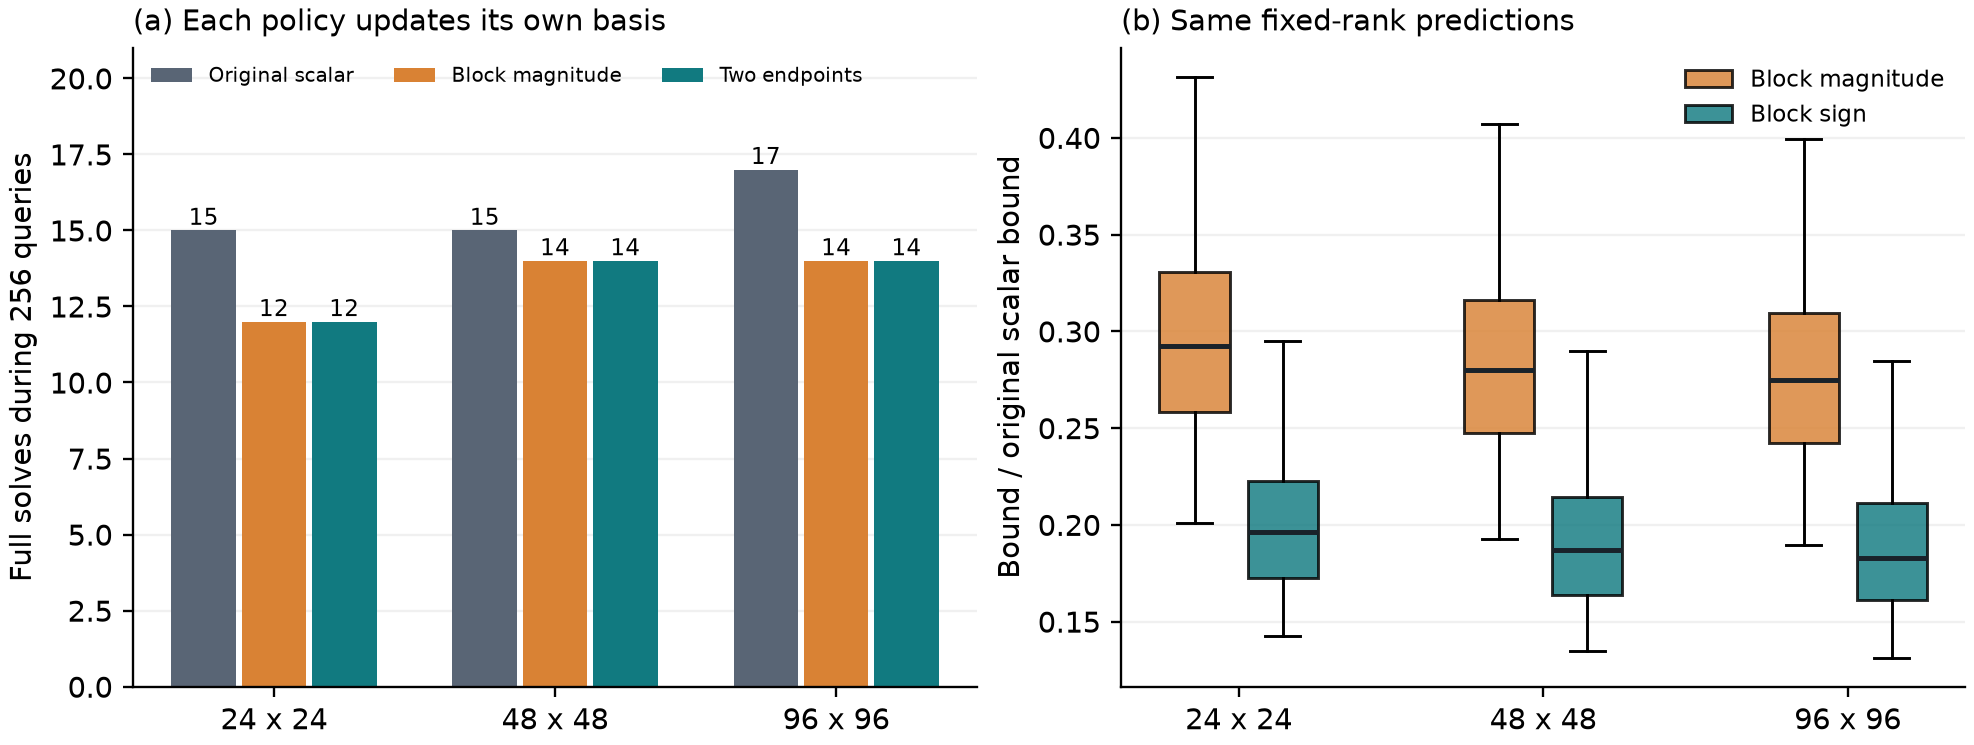
\includegraphics[width=\linewidth]{figures/residual_comparison.png}
\caption{左：在旧 256 参数流上各自更新基时，按网格统计真实回退次数。右：保持八维预测不动，显示新界与原标量界的逐例比值。箱体为四分位区间，中线为中位数，须至 $1.5$ 倍四分位距内的极值。双端点与单端符号在这些固定预测上重合。}
\end{figure}
\begin{table}[ht]\centering\small
\caption{完整策略本机部署耗时（秒），三次顺序运行的中位数。计入训练、模板准备、预测、判据、回退与更新，不含事后参照误差和模型研究时间。单次模板预处理的实测时间分摊到每次独立部署。}
\begin{tabular}{rrrr}\toprule
网格 & 原解析标量 & 分块正负 & 双端点\\\midrule
$24^2$ & 0.0487 & 0.0486 & 0.0512\\
$48^2$ & 0.1224 & 0.1287 & 0.1356\\
$96^2$ & 0.5917 & 0.5790 & 0.6159\\\bottomrule\end{tabular}
\end{table}

双端点少做了 7 次完整求解，但要在两端预计算 32 个响应模板，并在每次查询读出和组合这些响应。本次三个网格上双端点的总耗时均高于原判据；模块之间的毫秒差异受机器负载影响。选择较复杂的界，应同时考虑能节省多少完整求解和这些额外读数的成本。旧项目中约 $4.46$ 至 $5.39$ 倍的加速比较的是旧自适应求解和完整求解，并不衡量本次替换误差界的收益。

\paragraph{哪些结论可以推广？}
式~\eqref{eq:chain-new} 是针对上述离散算子在精确算术下的全参数不等式。大网格程序用普通双精度计算残差和端点模板，没有使用有向舍入；因此数值统计支持该实现的一致性，不能给双精度输出赋予机器认证含义。用独立网格和残差图样考察空间块的尺度，以及为计算出的局部端点增加显式舍入余量，是把这套方法移到更大模型时仍需处理的两个具体问题。
